\indent\underline{\textbf{Ejercicio 1}}\\
\textcolor{green}{[Programación]} Para el proceso de Markov de recompensas (MRP) de la figura~\ref{fig:grafo_ej_1}, calcular los valores de los estados de forma iterativa con los siguientes algoritmos y compare sus convergencias.
Considere factor de descuento $\gamma < 0.9$.\\

\begin{figure}[H]
    \centering
    \begin{tikzpicture}[->, >=stealth', auto, semithick, node distance=2cm]
        % Nodes
        \node[circle, draw] (s1) {$s_1$};
        \node[circle, draw, right=of s1] (s2) {$s_2$};
        % Arrows
        \path (s1) edge[bend left=60] node {R=1} (s2)
              (s2) edge[bend left=60] node[align=center] {R=2 \\ $p(s_2 \mid s_1) = 1$ \\ $p(s_1 \mid s_2) = 1$} (s1);
    \end{tikzpicture}
    \caption{Grafo de transición de estados}\label{fig:grafo_ej_1}
\end{figure}


\begin{itemize}
    \item Actualizar todos los valores a la vez por iteración: $v_{k+1} = r + \gamma P v_k$, con $v_k\, r$ siendo los vectores de valores y recompensas, respectivamente; y $P$ la matriz de probabilidades de transición.
    \item Actualizar los valores de un estado por vez \textit{(in place)}: $v_{k+1}(s') = r(s') + \gamma v_k(s)$, con $v_k(s)$ y $r(s')$ siendo los valores y recompensas correspondientes a los estados $s$ y $s'$, respectivamente.
\end{itemize}

\indent\underline{\textbf{Solución}}\\

Sea, $P$ la matriz de probabilidades de transición:

\[
  P = \begin{bmatrix} 0 & 1 \\ 1 & 0 \end{bmatrix}
\]

Sea $r$ el vector de recompensas:

\[
  r = \begin{bmatrix} 1 \\ 2 \end{bmatrix}
\]

A continuación los resultados de los valores de los estados para $\gamma \in [0, 0.9)$ usando los métodos \textit{iterativo} e \textit{in place}.

\paragraph{Método \textit{iterativo}} Se calculó el vector de valor $v_{k+1}$ usando el cálculo iterativo con la librería \texttt{numpy} de Python\footnotemark.
La figura~\ref{fig:iter_gamma_vk} muestra los valores de $v_{k+1}$ y la figura~\ref{fig:iter_gamma_iter} muestra el número de iteraciones necesarias para converger, ambas para $\gamma \in [0, 0.9)$.

\footnotetext{Se una tolerancia de $10^{-6}$ y un máximo de $1000$ iteraciones.}

La figura~\ref{fig:iter_gamma} muestra los resultados para el método \textit{iterativo}.

\begin{figure}[H]
    \centering
    \begin{subfigure}[H]{0.45\textwidth}
        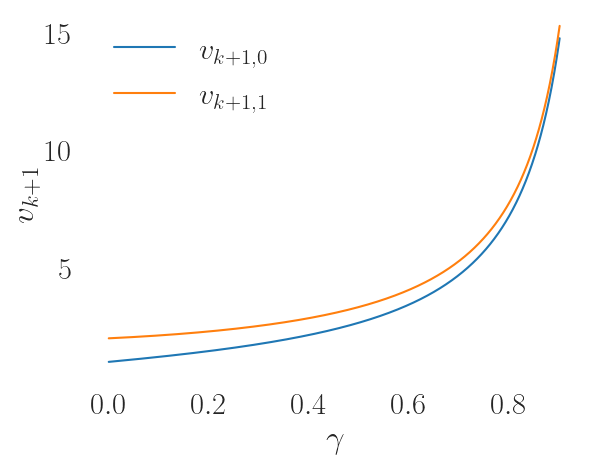
\includegraphics[width=\textwidth]{../img/gamma_v_k}
        \caption{Vector de valores}
        \label{fig:iter_gamma_vk}
    \end{subfigure}
    \begin{subfigure}[H]{0.45\textwidth}
        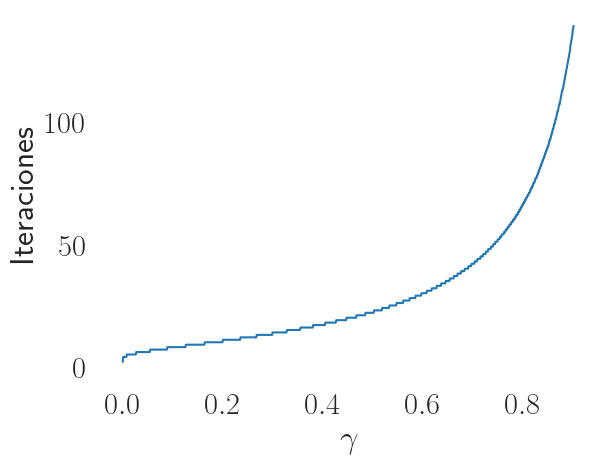
\includegraphics[width=\textwidth]{../img/gamma_iters}
        \caption{Número de iteraciones para converger}
        \label{fig:iter_gamma_iter}
    \end{subfigure}
    \caption{Resultados del método \textit{iterativo}}\label{fig:iter_gamma}
\end{figure}

\paragraph{Método \textit{in place}} Se calculó el vector de valor $v_{k+1}$ usando el cálculo iterativo con la librería \texttt{numpy} de Python\footnotemark.
La figura~\ref{fig:inplace_gamma_vk} muestra los valores de $v_{k+1}$ y la figura~\ref{fig:inplace_gamma_iter} muestra el número de iteraciones necesarias para converger, ambas para $\gamma \in [0, 0.9)$.

\footnotetext{Se fijó una tolerancia de $10^{-6}$ y un máximo de $1000$ iteraciones.}

La figura~\ref{fig:inplace_gamma} muestra los resultados para el método \textit{in place}.

\begin{figure}[H]
    \centering
    \begin{subfigure}[H]{0.45\textwidth}
        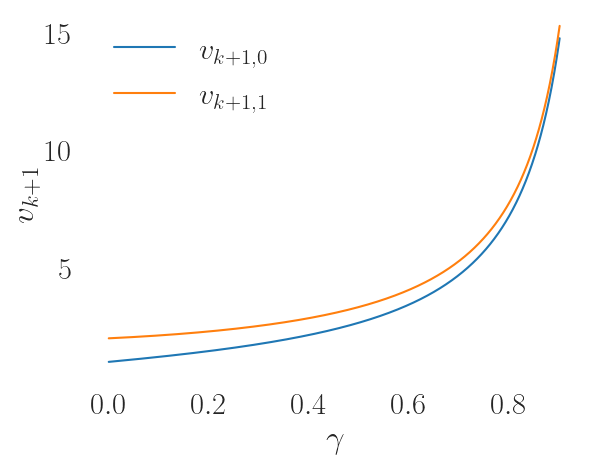
\includegraphics[width=\textwidth]{../img/gamma_v_k}
        \caption{Vector de valores}
        \label{fig:inplace_gamma_vk}
    \end{subfigure}
    \begin{subfigure}[H]{0.45\textwidth}
        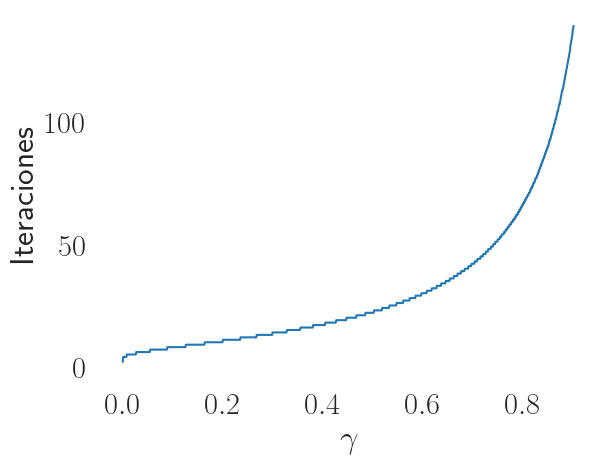
\includegraphics[width=\textwidth]{../img/gamma_iters}
        \caption{Número de iteraciones para converger}
        \label{fig:inplace_gamma_iter}
    \end{subfigure}
    \caption{Resultados del método \textit{inplace}}\label{fig:inplace_gamma}
\end{figure}


\indent\underline{\textbf{Conclusiones}}\\
No existe una diferencia significativa entre los métodos \textit{iterativo} e \textit{in place} para valores de $\gamma \in [0, 0.9)$.
A continuación se presentan las conclusiones de los resultados obtenidos.

\paragraph{Vector de valores $v_{k+1}$}
Las figuras~\ref{fig:iter_gamma_vk} y~\ref{fig:inplace_gamma_vk} muestran los valores de $v_{k+1}$ para $\gamma \in [0, 0.9)$ para los métodos \textit{iterativo} e \textit{in place}, respectivamente.
De las figuras se concluye,

\begin{itemize}
    \item Ambos métodos mostraron una rápida convergencia cuando $\gamma \approx 0$, dando como resultado $v_{k+1} = r = \begin{bmatrix} 1 \\ 2 \end{bmatrix}$.
    \item Los valores de $v_{k+1}$ aumentan de forma exponencial a medida que $\gamma$ aumenta.
    \item Conforme $\gamma \rightarrow 0.9$, los métodos convergen a los valores teóricos $v = \begin{bmatrix} 14.74 \\ 15.26 \end{bmatrix}$.
\end{itemize}

\paragraph{Iteraciones}
Las figuras~\ref{fig:iter_gamma_iter} y~\ref{fig:inplace_gamma_iter} muestran el número de iteraciones necesarias para converger para $\gamma \in [0, 0.9)$ para los métodos \textit{iterativo} e \textit{in place}, respectivamente.
De las figuras se concluye,

\begin{itemize}
    \item Las iteraciones necesarias para converger aumentan de forma exponencial a medida que $\gamma$ aumenta.
    \item Conforme $\gamma \rightarrow 0.9$, se requieren más iteraciones para converger, lo que se traduce en un mayor tiempo de cómputo.
\end{itemize}

\paragraph{Implementación}En cuanto a la implementación de ambos métodos, la diferencia entre el método \textit{iterativo} e \textit{in place} radica en que el segundo no requiere de una matriz de transición $P$.
Desde una perspectiva computacional el método \textit{in place} es más eficiente, ya que no requiere de una matriz de transición.
También es útil en escenarios en los que la matriz de transición no es conocida, como en el caso de un agente que interactúa con un entorno desconocido.

\line(1,0){\textwidth}
